% Template latex non officiel pour rapport de TP EEA.
% C'est un template pour thèse que j'ai adapté et 
% auquel j'ai ajouté des éléments au fil du temps pour mes rapports de TP.
% En cas de problèmes n'hésites pas a me contacter.
% David Tocaven
% david.tocaven@gmail.com


%%% /!\ /!\ /!\ /!\ /!\ /!\
% Se compile avec PDFLatex
%%% /!\ /!\ /!\ /!\ /!\ /!\
%%=================================================%%
%%						MAIN
%%=================================================%%


\documentclass[a4paper]{report}

%====================== PACKAGES ======================
\usepackage{bbold}
\usepackage{soul}				% souligner
\usepackage{dsfont}
\usepackage[french]{babel}		% Pour avoir le document en français
\usepackage[utf8x]{inputenc}	% Encodage du document
\usepackage{float}				% Pour gérer les positionnement d'images
\usepackage{amsmath}
\usepackage{mathrsfs}			% Pour les lettres calligraphiques équation
\usepackage{url}				% Pour faire des hyperliens vers le web
\usepackage{color}
% pour les informations sur un document compilé en PDF et les liens externes / internes
\usepackage{hyperref}			% Pour faire des hyperliens
\usepackage{array}				% Pour faire des tableaux
\usepackage{tabularx}
% pour utiliser 		% floatbarrier
%\usepackage{placeins}
%\usepackage{floatrow}
\usepackage{setspace}			% Espacement entre les lignes
\usepackage{abstract}			% Modifier la mise en page de l'abstract
\usepackage[T1]{fontenc}		% Police et mise en page (marges) du document
\usepackage[top=2cm, bottom=2cm, left=2cm, right=2cm]{geometry}
\usepackage{pdfpages}			% pour inclures des pdf comme des images
\usepackage{subfig}				% Pour les galerie d'images
\usepackage{listings}			% pour inclure du code dans le doc
\usepackage{soul}				% Pour surligner
\usepackage{enumitem}

\sethlcolor{grisclair}
\definecolor{darkgreen}{RGB}{0,100,0}
%% Titre import from last TP
\usepackage{titlesec, blindtext, color}	
\definecolor{gray75}{gray}{0.75}
\newcommand{\hsp}{\hspace{20pt}}
\titleformat{\chapter}[hang]{\Huge\bfseries}{\thechapter\hsp\textcolor{gray75}{|}\hsp}{0pt}{\Huge\bfseries}

%====================== INFORMATION ET REGLES ======================

%rajouter les numérotation pour les \paragraphe et \subparagraphe
\setcounter{secnumdepth}{4}
\setcounter{tocdepth}{4}

\hypersetup{							% Information sur le document
pdfauthor = { NOM },				% Auteurs
pdftitle = {Matière - Titre - Sujet },		% Titre du document
pdfsubject = {matière},		% Sujet
pdfkeywords = {},				% Mots-clefs
pdfstartview={FitH}}					% ajuste la page à la largueur de l'écran
%pdfcreator = {MikTeX},% Logiciel qui a crée le document
%pdfproducer = {}} % Société avec produit le logiciel

\newcounter{cpt1}						% Compteur pour les n° de ligne dans les prog de l'annexe1
\newcommand\increm{\arabic{cpt1}\addtocounter{cpt1}{1}}
%initialisation de l'intégrateur de language C



%======================== DEBUT DU DOCUMENT ========================

\begin{document}

%\lstset{
%  language=C,                	  % choose the language of the code
%  numbers=left,                   % where to put the line-numbers
%  stepnumber=1,                   % the step between two line-numbers.
%  numbersep=5pt,                  % how far the line-numbers are from the code
%  backgroundcolor=\color{white},  % choose the background color. You must add \usepackage{color}
%  showspaces=false,               % show spaces adding particular underscores
%  showstringspaces=false,         % underline spaces within strings
%  showtabs=false,                 % show tabs within strings adding particular underscores
%  tabsize=2,                      % sets default tabsize to 2 spaces
%  captionpos=b,                   % sets the caption-position to bottom
%  breaklines=true,                % sets automatic line breaking
%  breakatwhitespace=true,         % sets if automatic breaks should only happen at whitespace
%  title=\lstname,                 % show the filename of files included with \lstinputlisting;
%}
%régler l'espacement entre les lignes
\newcommand{\HRule}{\rule{\linewidth}{0.5mm}}


%page de garde
%%=================================================%%
%%						TITRE DU DOCUMENT (1 PAGE)
%							  Pas totalement fini
%%=================================================%%

\begin{titlepage}
\begin{center}

% Upper part of the page. The '~' is needed because only works if a paragraph has started.


\includegraphics[width=0.60\textwidth]{./page_de_garde/logo_ups.png}~\\[1cm]

\textsc{\LARGE Université Paul Sabatier}\\[1.5cm]

\textsc{\Large \bf Conception des systèmes temps réel }\\[0.5cm]

% Title
\HRule \\[0.4cm]

{\huge \bfseries  TP : \textsc{Rapport de conception UML -- SysML} }

\HRule \\[1.5cm]

% Author and supervisor
\begin{minipage}[t]{0.4\textwidth}
\begin{flushleft} \large
\emph{Auteurs:}\\ \vspace{3mm}
Dhouha \textsc{Ajroud}\\
Léonard \textsc{Herrero}\\
Julien \textsc{Rey}\\
Lucien \textsc{Rakotomalala}\\
David \textsc{Tocaven}
\end{flushleft}
\end{minipage}
\begin{minipage}[t]{0.58\textwidth}
\begin{flushright} \large
\emph{Encadrant:}\\ \vspace{3mm}
\textbf{ Vincent \textsc{Albert}}\\
\textbf{Pascal \textsc{Berthou}}\\
\vfill
\end{flushright}
\end{minipage}
\newline
\newline

% une éventuelle image
%\includegraphics[width=.6\textwidth]{./page_de_garde/BACDO_schema.pdf}~\\[1cm]

\vfill
% logo fsi & eea
\begin{tabular}{cc}
   
\includegraphics[height=2cm]{./page_de_garde/logo_fsi.png} \hspace{2cm} &
    \hspace{2cm}
   
\includegraphics[height=2cm]{./page_de_garde/logo_eea.jpg} \\
\end{tabular}

% Bottom of the page
{\large \today}

\end{center}
\end{titlepage}
	

%page blanche
\newpage
~
\tableofcontents
\thispagestyle{empty}
\setcounter{page}{0}
%ne pas numéroter le sommaire


%espacement entre les lignes d'un tableau
\renewcommand{\arraystretch}{1.5}

%====================== INCLUSION DES PARTIES ======================
%
%~
\thispagestyle{empty}
%recommencer la numérotation des pages à "1"
\setcounter{page}{0}

\chapter*{Introduction}
\addcontentsline{toc}{chapter}{Introduction}
\label{chap:Intro}	% Importation de introduction.tex

\chapter{Analyse du besoin}

\section{Diagramme Cas d'utilisation}	% diagrame
% Je pense que ça doit être là
\begin{figure}[!ht]
\centering
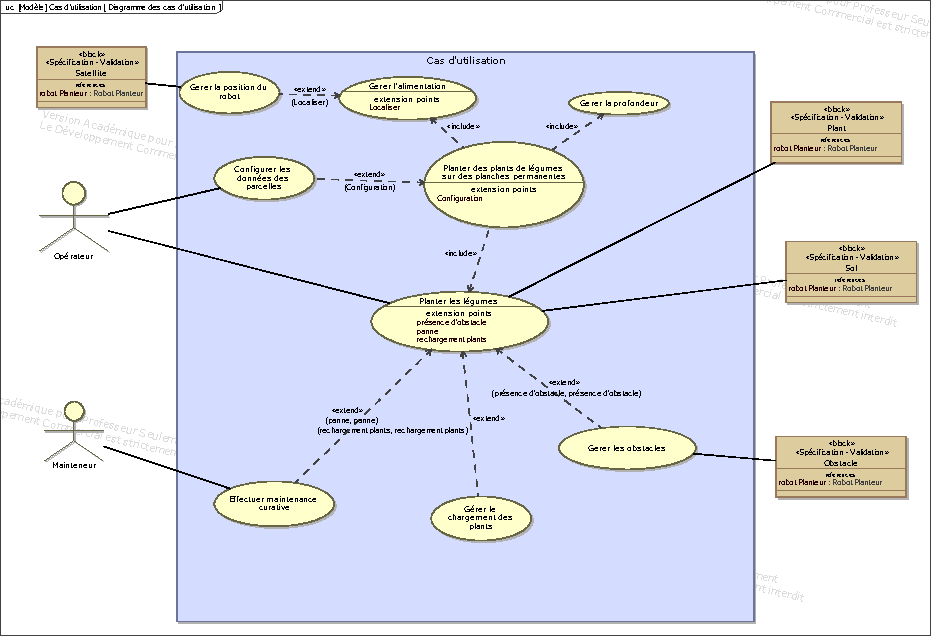
\includegraphics[width=.7\textwidth]{./I/images/casUtilisation.pdf}
\caption{Diagramme des cas d'utilisation}\label{fig:diagUC}
\end{figure} 
Nous avons placé dans l'ensemble de nos cas d'utilisation deux acteurs qui peuvent se dissocier : l'opérateur et le mainteneur. de manière assez naturelle, nous avons placé au centre des cas "Planter les légumes", point névralgique du système. De ce centre dépend plusieurs autres utilisations de notre système comme effectuer des maintenances, gestion des obstacles et des plants et enfin toute la partie de configuration du système.

\section{Scénarios et diagramme de séquence}
Nous avons fait le choix de ne traiter que 3 cas d'utilisation en scénarios et diagrammes de séquence.

\paragraph*{Cas d'utilisation 1 : Planter des choux}
Après que l’opérateur ait positionné le robot en position initiale, chargé 240 plants sur le robot et configuré la parcelle, il le met en marche.
Le robot avance, s’arrête sur la zone a planter puis charge un plant dans chaque buses. Les buses se positionnent sur la zone à planter, descendent, perforent le sol puis s'ouvrent pour laisser tomber les plants. Le cycle recommence jusqu’à arrivé en bout de planche ou le robot effectue une translation vers la droite pour se placer en bout de la planche suivante et répéter le cycle de plantation jusqu’à arrivé en bout de parcelle ou que le stock de plants soit vide.\begin{center}
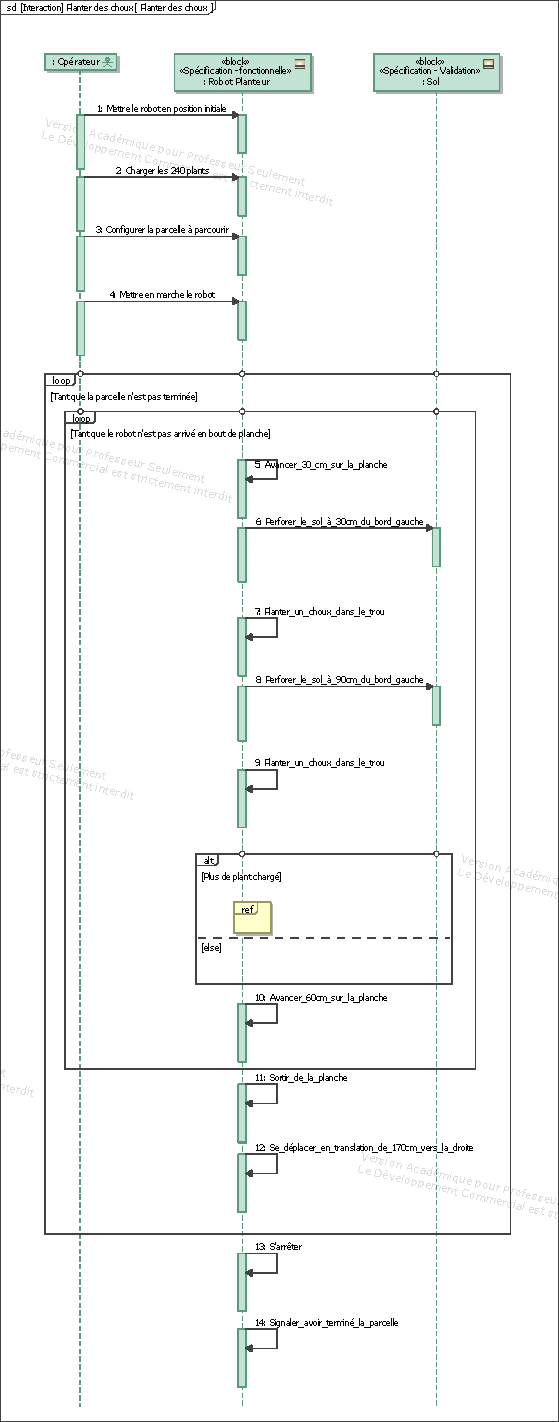
\includegraphics[width=.5\textwidth]{./I/images/planterChoux.pdf}
\captionof{figure}{Diagramme de séquence : Planter des choux}\label{fig:diagSeqPlanterChoux}
\end{center} 

\paragraph*{Cas d'utilisation 2: Gérer le chargement des plant}
Quand le robot détecte que son stock est vide, il enregistre son état actuel, il avertie ensuite l’opérateur à l'aide d'un signal physique puis se dirige en bout de planche. L’opérateur recharge le robot en plants, valide le chargement et le robot reprend la position sauvegarder précédemment et continue son cycle normal.%% Vraiment désolé, j'ai été obligé de passer cmme sa pour la faire tenir en place
\begin{center}
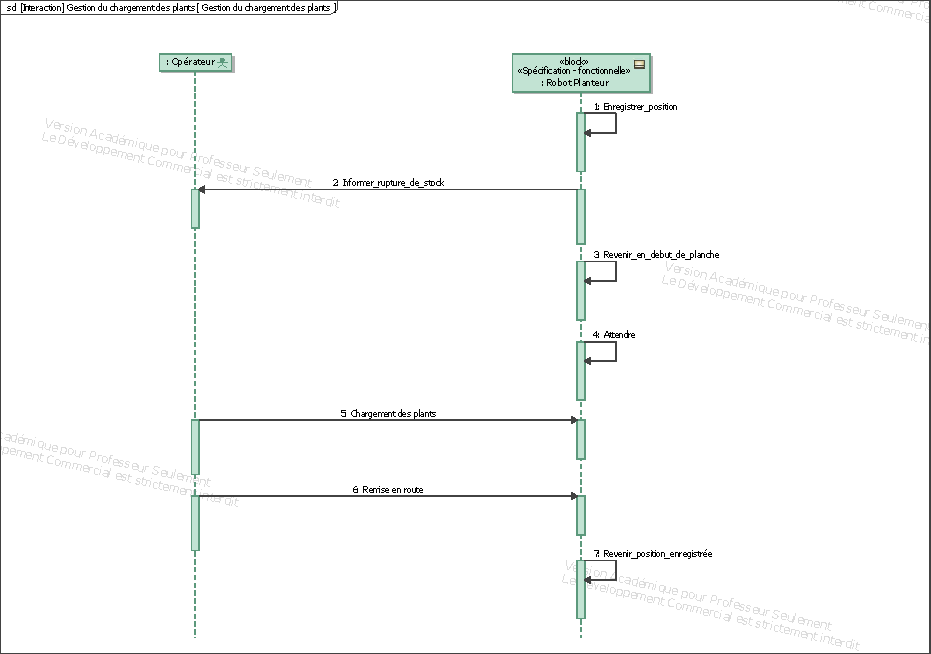
\includegraphics[width=.5\textwidth]{./I/images/gestionChargementPlant.pdf}
\captionof{figure}{Diagramme de séquence : Gestion du chargement des plants}\label{fig:diaggestionChargement}
\end{center} 


\paragraph*{Cas d'utilisation 3: Gérer les obstacles}
Lorsque un obstacle se présente devant le robot, il est détecté et le robot s'arrête. Il signale l'obstacle à l’opérateur à l'aide d'un signal physique. Pour que le robot reprenne son cycle normal l'obstacle ne doit plus être détecté par le robot et l’opérateur doit valider la remise en marche. 

\begin{figure}[!ht]
\centering
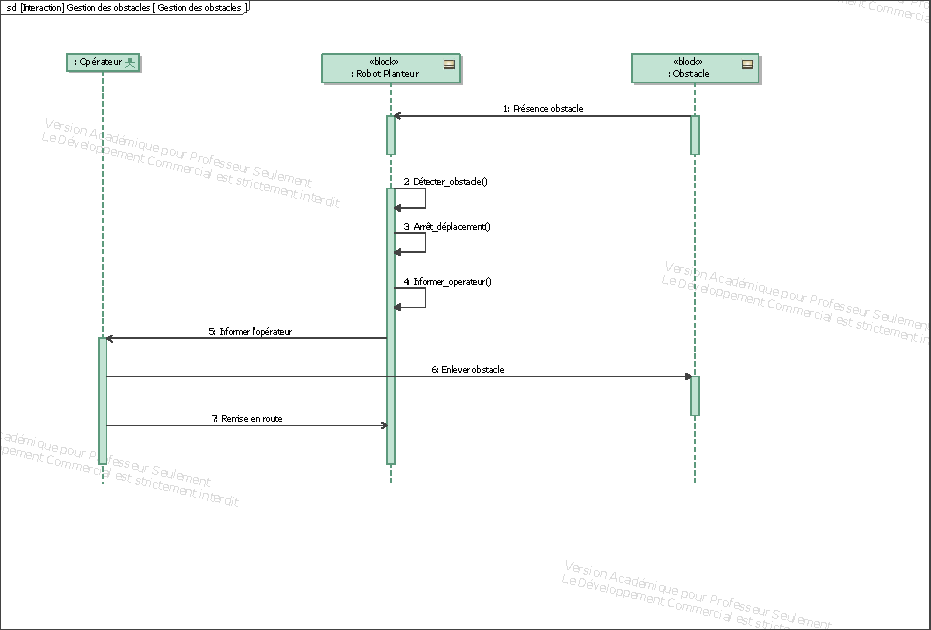
\includegraphics[width=.6\textwidth]{./I/images/gererObstacles.pdf}
\caption{Diagramme de séquence : Gérer les obstacles}\label{fig:diagSeqGereObstacle}
\end{figure}

\chapter{}


\chapter{Architecture}
Nous allons maintenant passer à la description de l'architecture de notre système en commençant par pour vous présenter l’architecture logique, suivi de l'architecture physique. Nous terminerons par l'observation des lien entre les exigences requises par notre Robot avec cette architecture.

\section{Architecture Logique}
Dans ce diagramme \ref{fig:architectureLogique}, nous avons encapsuler les fonctions primaires de notre Robot. Nous avons choisi de définir 9 \emph{Sous-systèmes logique} avec, comme bloc principal le Robot Planteur.
\begin{figure}[!ht]
\centering
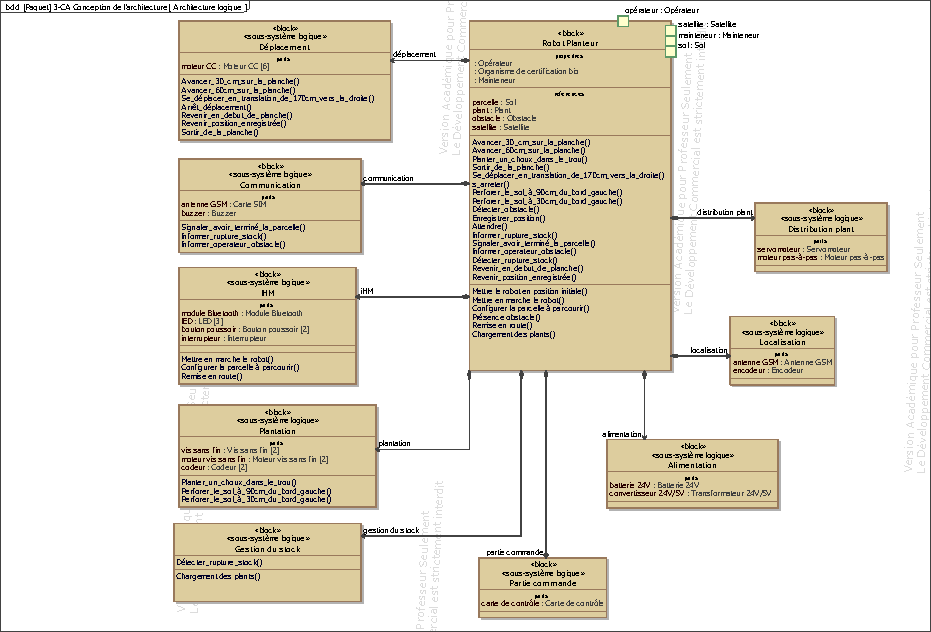
\includegraphics[width = \textwidth]{./III/images/SysML_Block_Definition_Diagram_3-CA_Conception_de_l_architecture_Architecture_logique.pdf}
\caption{Architecture Logique}\label{fig:architectureLogique}
\end{figure}
\subsection{Description des sous-systèmes logiques}
\paragraph*{Déplacement}
Ce \emph{Sous-système} doit permettre au robot d'avancer de manière précise sur la planche (30 cm ou 60 cm pour planter les différents plants), se sortir de la planche sans toucher et donc, en effectuant la translation aussi à disposition dans ce \emph{Sous-système}. Enfin, il doit permettre au robot d'être être capable de s'arrêter très rapidement et rester immobile après cet arrêt. 
\paragraph*{Communication}
Il permet d'informer l'opérateur si le robot se retrouve perturbé dans sa mission : un obstacle, une rupture de stock ou une fin du travail demandé. 
\paragraph*{IHM}
Le \emph{Sous-système} \textbf{Interface Homme Machine} doit permettre toute la configuration du système par l'opérateur. Il contient donc naturellement les fonctions de configuration et de mise en route. 
\paragraph*{Plantation}
Comme son nom l'indique, il doit permettre d'effectuer la fonction principale du robot. Toute la partie de perforation des sols est contenu dans ce \emph{Sous-système}. 
\paragraph*{Gestion du stock}
Il englobe tous l'ensemble de fonctions qui vont permettre de détecter les ruptures de stock en plants, et ce donc contient un ensemble de capteurs que nous détaillons en architecture physique (\ref{fig:architecturePhysique}).  
\paragraph*{Partie Commande}
Toute la gestion numérique permettant la commande du Robot seront contenu dans ce \emph{Sous-système}. Il convient donc d'utiliser des cartes électroniques programmable pour la réalisation de ces fonctions.
\paragraph*{Alimentation}
Ce \emph{Sous-système} doit permettre l'alimentation électrique de tout le robot. Il doit donc être suffisant puissant pour satisfaire en énergie toute les fonctions motrices du robot.
\paragraph*{Localisation}
Toute la gestion de l'emplacement du Robot sera contenu dans ce \emph{Sous-système}. Elle nécessitera un encodage pour permettre la communication des données avec plusieurs autres \emph{Sous-systèmes}.
\paragraph*{Distribution plant} 
Ce dernier \emph{Sous-système} va permettre l'approvisionnement en plants au bec du robot.  

\section{Architecture Physique}
Dans cette représentation \ref{fig:architecturePhysique}, nous avons établi le matériel qui sera utilisé pour remplir les fonctions logiques décrites plus tôt. Nous avons laissé libre choix sur les moteurs CC et les servomoteurs, sur les Vis et les moteurs associés, sur les parties communicantes, sur les batteries et transformateur et les composants de l'IHM. 
\begin{figure}[!ht]
\centering
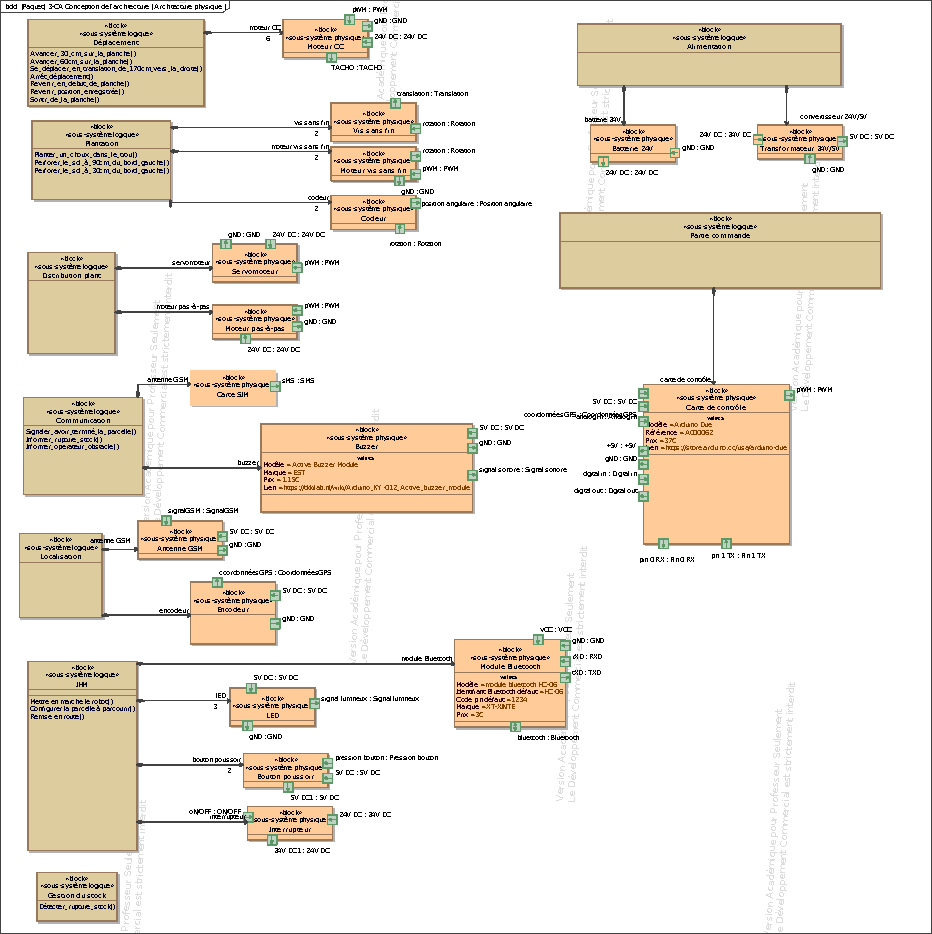
\includegraphics[width = \textwidth]{./III/images/SysML_Block_Definition_Diagram_3-CA_Conception_de_l_architecture_Architecture_physique.pdf}
\caption{Architecture Physique}\label{fig:architecturePhysique}
\end{figure}

\section{Traçabilité de la conception}
Chaque composant a, dans ce diagramme \ref{fig:tracabiliteConception}, été relié à un besoin. Nous remarquons, dans le cas de la \emph{carte de contrôle}, qu'elle est relié à tout les besoins : il s'agit d'une partie critique de notre système. La réalisation de cette partie devra demander beaucoup de précisions.
\begin{figure}[!ht]
\centering
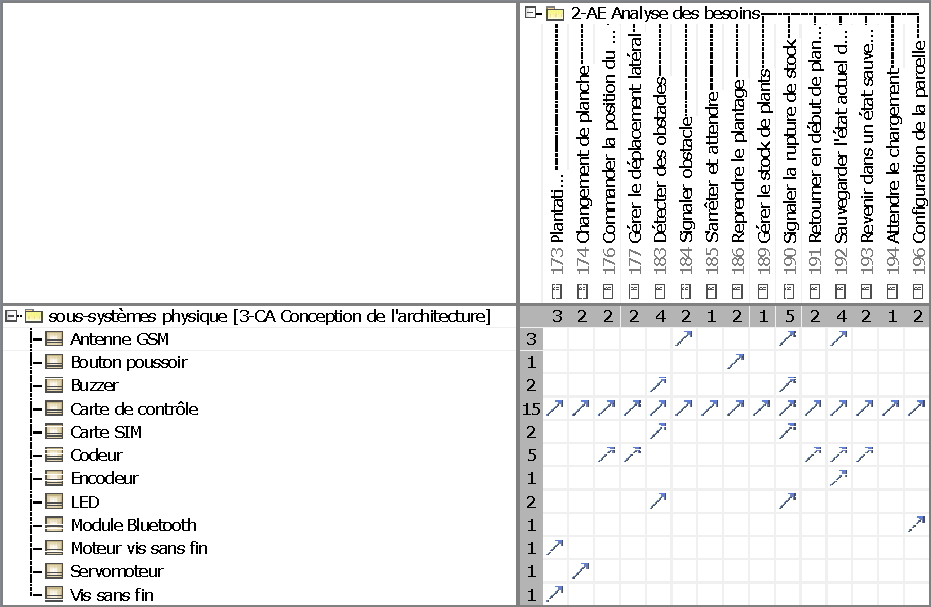
\includegraphics[width = \textwidth]{./III/images/Dependency_Matrix_3-CA_Conception_de_l_architecture_Tracabilite_conception.pdf}
\caption{Traçabilité de conception}\label{fig:tracabiliteConception}
\end{figure}


%\chapter{Description du Matériel Utilisé}

\section{Arduino DUE}

\section{}



%\input{./V/chap5.tex}

%\input{./VI/chap6.tex}

%\input{./conclusions/conclusions.tex}

\chapter{Conclusion}



%Ne pas numéroter cette partie
\part*{Annexes}
%Rajouter la ligne "Annexes" dans le sommaire
\addcontentsline{toc}{part}{Annexes}

\chapter*{Annexe 1 - TITRE}
\addcontentsline{toc}{chapter}{TITRE}
%\setcounter{section}{0}
% **********************************
\addcontentsline{toc}{section}{TITRE}
\label{Annex:NOM_FICHIER}
\lstset{
  language=Matlab,                	  % choose the language of the code
  basicstyle=\ttfamily,
  numbers=left,                   % where to put the line-numbers
  stepnumber=1,                   % the step between two line-numbers.
  numbersep=5pt,                  % how far the line-numbers are from the code
  backgroundcolor=\color{white},  % choose the background color. You must add \usepackage{color}
  commentstyle = \color{darkgreen},
  showspaces=false,               % show spaces adding particular underscores
  showstringspaces=false,         % underline spaces within strings
  showtabs=false,                 % show tabs within strings adding particular underscores
  tabsize=2,                      % sets default tabsize to 2 spaces
  captionpos=b,                   % sets the caption-position to bottom
  breaklines=true,                % sets automatic line breaking
  breakatwhitespace=true,         % sets if automatic breaks should only happen at whitespace
  %caption=exo1.m,                 % show the filename of files included with \lstinputlisting;
  literate={á}{{\'a}}1 {è}{{\`e}}1 {é}{{\'e}}1,
}
%\lstinputlisting{./annexes/annexe1/NOMFICHIER.m} %{language = MAtlab}
\chapter*{Annexe 2 - TITRE}
\addcontentsline{toc}{chapter}{Annexe 2 - TITRE}
\setcounter{section}{0}
\setcounter{subsection}{0}
% **********************************
	%


\newpage

%récupérer les citation avec "/footnotemark"
\nocite{*}

%%choix du style de la biblio
%\bibliographystyle{unsrt}
%%inclusion de la biblio
%\bibliography{bibliographie}
%%voir wiki pour plus d'information sur la syntaxe des entrées d'une bibliographie

\end{document}

